\begin{apartats}

\apartat[1,25]{1}
Troba totes les asímptotes de la funció
\[
f(x)=\frac{x+2}{x^2-2x-3} .
\]

\begin{solucio}
\textbf{Verticals}: el denominador és $(x-3)(x+1)$, que s'anul·la en $x=3$ i en $x=-1$, i el numerador
no s'hi anul·la ($5$ i $1$). En $x=3$ els laterals valen $-\infty$ i $+\infty$, i en $x=-1$, $+\infty$
i $-\infty$: asímptotes verticals $\boxed{x=3}$ i $\boxed{x=-1}$.\\
\textbf{Horitzontal}: el grau del numerador és més petit que el del denominador, i
$\lim_{x\to\pm\infty}f(x)=0$: asímptota horitzontal $\boxed{y=0}$. Per tant, no n'hi ha cap d'obliqua.
\end{solucio}

\begin{nomesllarg}
\apartat{0,75}
Troba totes les asímptotes de la funció
\[
g(x)=\frac{x^2-4x+5}{x-2} .
\]

\begin{solucio}
\textbf{Vertical}: $x=2$, perquè el denominador s'hi anul·la i el numerador val $1\neq0$.\\
\textbf{Obliqua}: dividint, $\dfrac{x^2-4x+5}{x-2}=x-2+\dfrac{1}{x-2}$, i el terme que sobra tendeix a
$0$: asímptota obliqua $\boxed{y=x-2}$. No hi ha asímptota horitzontal.
\end{solucio}
\end{nomesllarg}

\begin{tria}{asimptotes-tasca}
\itemtria{original}{0,75}{1,25}
Dibuixa la gràfica d'una funció que tingui domini $\mathbb{R}\setminus\{-1\}$, asímptota vertical
$x=-1$ i asímptota obliqua $y=x$, i escriu-ne una expressió.

\begin{solucio}
Per exemple, $f(x)=x+\dfrac{1}{x+1}$: el domini és $\mathbb{R}\setminus\{-1\}$; en $x=-1$ els laterals
valen $-\infty$ (per l'esquerra) i $+\infty$ (per la dreta); i $f(x)-x=\dfrac{1}{x+1}\to0$ quan
$x\to\pm\infty$, de manera que $y=x$ és asímptota obliqua pels dos costats.
\begin{center}
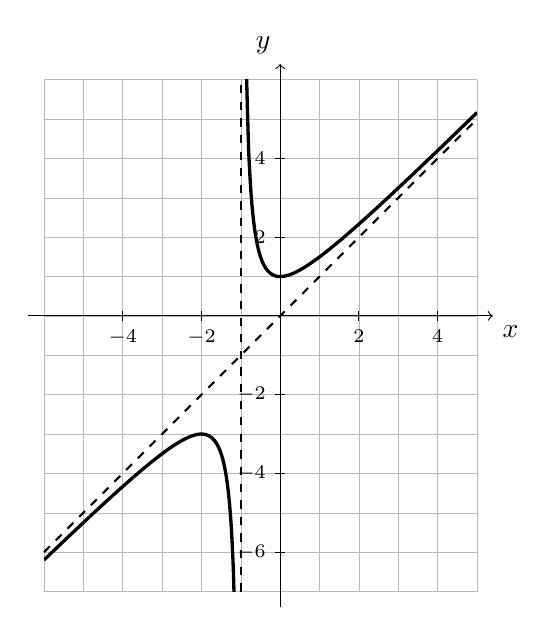
\begin{tikzpicture}[x=0.5cm,y=0.5cm]
  \draw[gray!55,very thin,step=1] (-6,-7) grid (5,6);
  \draw[->] (-6.4,0) -- (5.4,0) node[below right] {$x$};
  \draw[->] (0,-7.4) -- (0,6.4) node[above left] {$y$};
  \foreach \i in {-4,-2,2,4} \draw (\i,0.12) -- (\i,-0.12) node[below,font=\scriptsize] {$\i$};
  \foreach \j in {-6,-4,-2,2,4} \draw (0.12,\j) -- (-0.12,\j) node[left,font=\scriptsize] {$\j$};
  \draw[dashed,thick] (-1,-7) -- (-1,6);
  \draw[dashed,thick] (-6,-6) -- (5,5);
  \begin{scope}
    \clip (-6,-7) rectangle (5,6);
    \draw[\colorgrafica,very thick,domain=-6:-1.14,samples=100,smooth] plot (\x,{\x+1/(\x+1)});
    \draw[\colorgrafica,very thick,domain=-0.86:5,samples=100,smooth] plot (\x,{\x+1/(\x+1)});
  \end{scope}
\end{tikzpicture}
\end{center}
Qualsevol altra funció amb aquestes propietats també val.
\end{solucio}

\itemtria{branques-polinomi}{0,75}{1,25}
Estudia les branques infinites de la funció polinòmica
\[
p(x)=-x^3+2x^2+5 ,
\]
i justifica que no té cap asímptota. Passa el mateix amb qualsevol polinomi de grau més gran que $1$?

\begin{solucio}
$\lim_{x\to-\infty}p(x)=+\infty$ i $\lim_{x\to+\infty}p(x)=-\infty$: hi mana el terme de grau màxim,
$-x^3$.\\
\textbf{Verticals}: cap, perquè $p$ està definida i és contínua a tot $\mathbb{R}$.
\textbf{Horitzontals}: cap, perquè els límits a l'infinit no són finits. \textbf{Obliqües}: cap,
perquè $\dfrac{p(x)}{x}=-x^2+2x+\dfrac5x\to-\infty$ als dos costats, i el pendent no pot ser finit.\\
Passa el mateix amb qualsevol polinomi de grau $n\ge2$: $\dfrac{p(x)}{x}$ és de grau $n-1\ge1$ i
tendeix a $\pm\infty$. Les seves branques infinites són \textbf{parabòliques}, sense asímptota.
\end{solucio}
\end{tria}

\end{apartats}
